\documentclass[11pt,a4paper]{report}
\usepackage[utf8]{inputenc}
\usepackage[croatian]{babel}
\usepackage{amsmath, amsfonts, amssymb}
\usepackage{graphicx}
\usepackage{fancyhdr}
\usepackage{color}
\usepackage {tikz}
\usepackage{pgfplots}
\usetikzlibrary {positioning}
\usepackage{tocloft}
\usepackage[hidelinks]{hyperref}
\usepackage[section]{placeins}
\usepackage[final]{pdfpages}
\bibliographystyle{abbrv}%ieeetr, abbrv
\renewcommand{\cftsecleader}{\cftdotfill{\cftdotsep}}
\addto{\captionscroatian}{\renewcommand{\bibname}{Literatura}}

\usepackage[blocks]{authblk}% The option is for block layout

\newcommand{\kolegij}{}
\newcommand{\naslovRada}{Proračun i konstrukcija 1-stupnjskog reduktora s cilindričnim ravnim zubima \\ {\large Timski projektni zadatak}} 
\newcommand{\mailFriendlynaslovRada}{Konstrukcije - projektni zadatak}

%\author{
%Kristijan Cetina \\{\small JMBAG: 2424011721} \\ {\href{mailto:kcetina@politehnika-pula.hr?subject=\mailFriendlynaslovRada}{{\footnotesize kcetina@politehnika-pula.hr}}} \and 
%Stjepan Grgin \\{\small JMBAG: 0112005802} \\ {\href{mailto:sgrgin@politehnika-pula.hr?subject=\mailFriendlynaslovRada}{{\footnotesize sgrgin@politehnika-pula.hr}}} \and 
%Igor Mrkić \\{\small JMBAG: 0114017089} \\ {\href{mailto:imrkic@politehnika-pula.hr?subject=\mailFriendlynaslovRada}{{\footnotesize imrkic@politehnika-pula.hr}}}
%}


\author[1]{Kristijan Cetina}
\author[2]{Stjepan Grgin}
\author[3]{Igor Mrkić}

\affil[1]{\href{mailto:kcetina@politehnika-pula.hr?subject=\mailFriendlynaslovRada}{kcetina@politehnika-pula.hr} JMBAG: 2424011721}
\affil[2]{\href{mailto:sgrgin@politehnika-pula.hr?subject=\mailFriendlynaslovRada}{sgrgin@politehnika-pula.hr} JMBAG: 0112005802}
\affil[3]{\href{mailto:imrkic@politehnika-pula.hr?subject=\mailFriendlynaslovRada}{imrkic@politehnika-pula.hr} JMBAG: 0114017089}



%\title{\kolegij \\ \naslovRada}
\title{\naslovRada}
\date{Pula, \today}

\begin{document}
\pgfplotsset{width=\textwidth,compat=newest}

\begin{titlepage}
\clearpage
\begin{center}
\begin{Huge}
POLITEHNIKA PULA\\
\end{Huge}
\begin{LARGE}
Visoka tehničko-poslovna škola s p.j.\\
Stručni studij politehnike\\
\end{LARGE}
\end{center}
\vspace{3cm}
{\let\newpage\relax\maketitle}
\thispagestyle{empty}
\vfill
\begin{abstract}
U ovom radu predstavljamo proračun strojnog sklopa - 1-stupanjskog reduktora zajedno s pripradajućim vratilima i ležajevima koji je zadan kao sastavni dio kolegija Konstrukcije.
\end{abstract}
\end{titlepage}
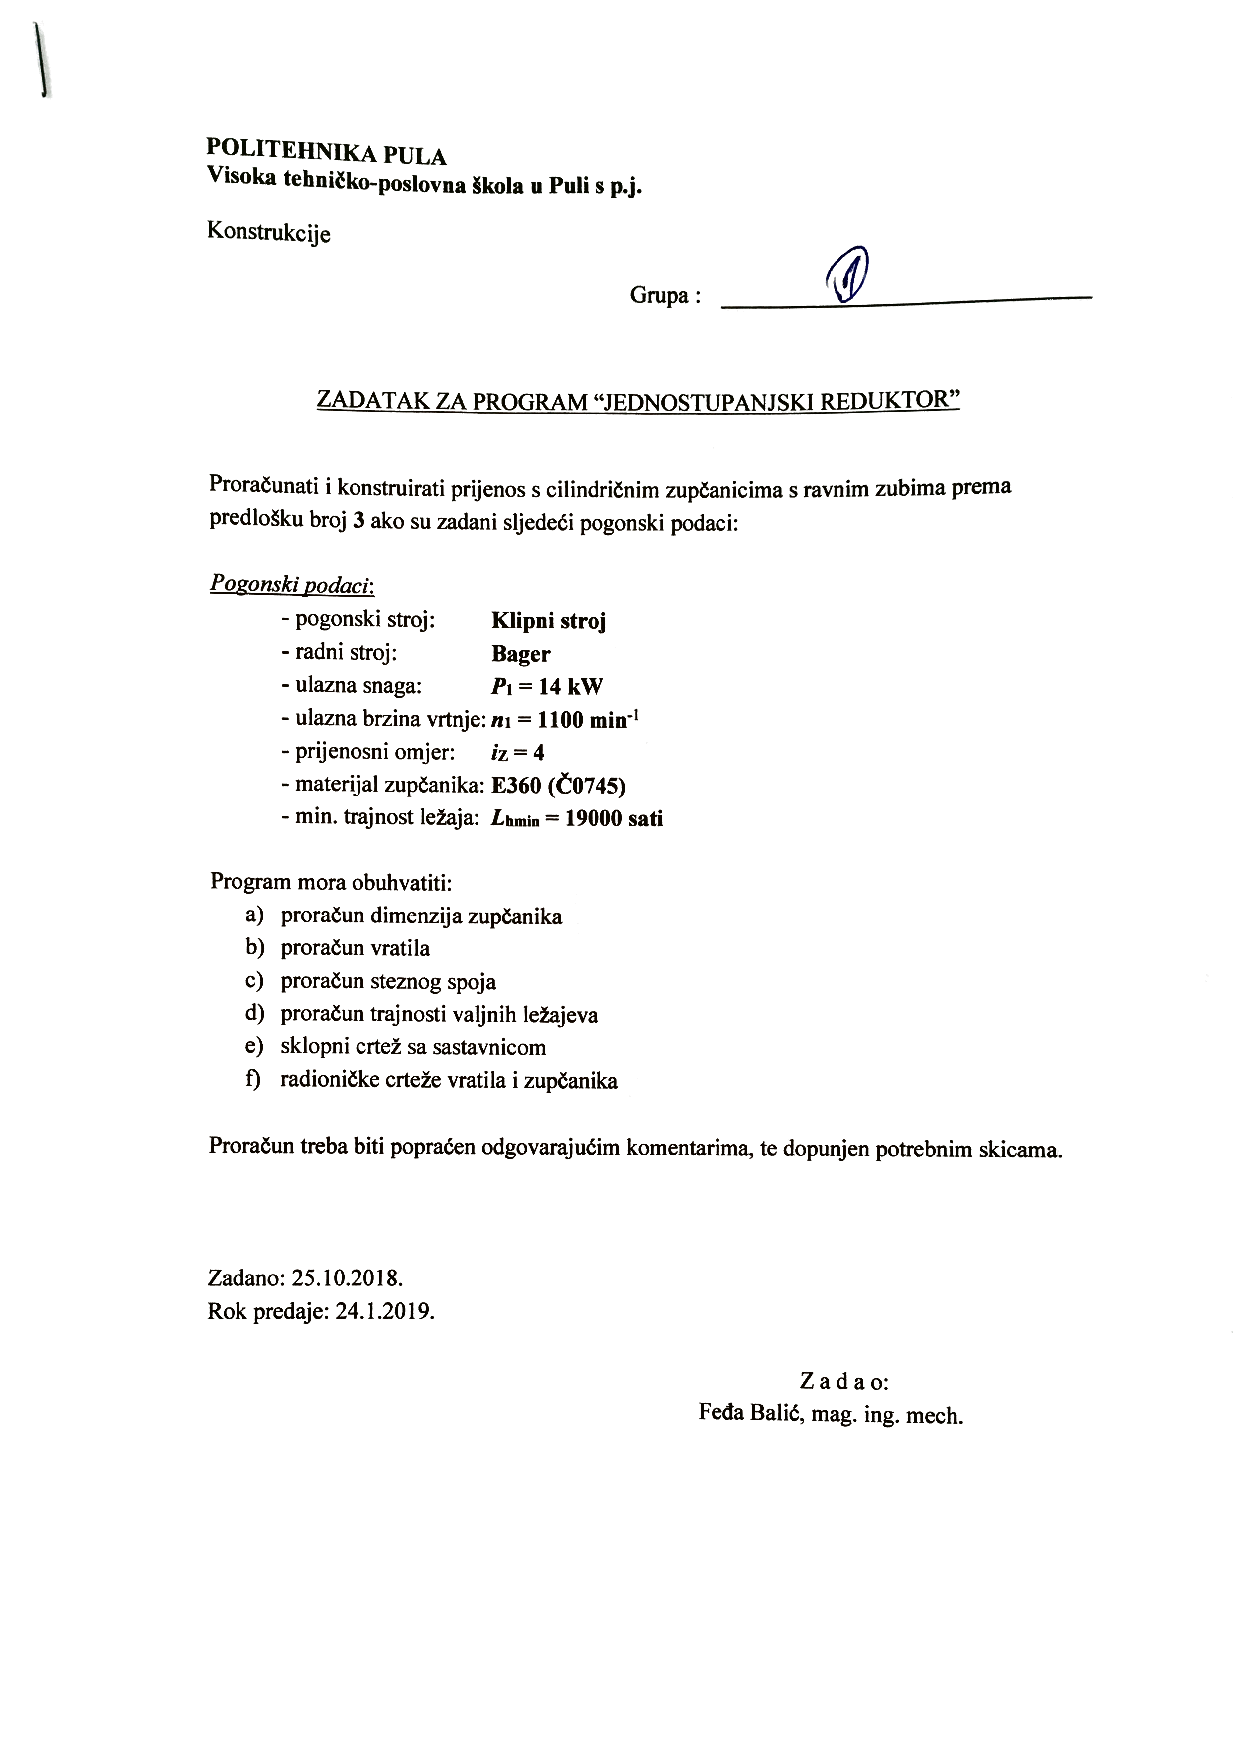
\includepdf[fitpaper]{TimskiProjektniZadatak.pdf}
\tableofcontents
%\listoftables	%ako ih ima puno prebaci na kraj dokumenta
%\listoffigures	%ako ih ima puno prebaci na kraj dokumenta

%Ovdje kreće rad ili može se koristiti
%\input{filename} (da nastavi pisati kako da je copy/paste) ili
%\include{filename} (da ubaci na novu stranicu. Ok za nova poglavlja i sl)
\chapter{Opis zadatka i ograničenja}
\section{Uvod}
Ovaj projektni zadatak nastao je kao obavezni zadatak u sklopu kolegija Konstrukcije koji se održava pod vodstvom Milenka Jokića, dipl.ing., predavača na stručnom studiju politehnike pri Politehnici Pula te asistenciju Feđe Balića, mag. ing. mech.

Prema zadanom predlošku (predložak 3) i zadanim podacima konstriran je 1-stupanjski reduktor s cilindričnim ravnim zubima.
Uvedena su sljedeća pojednostavljena i zanemareni sljedeći dijelovi proračuna:
\begin{itemize}
\item kontrolni proračun
\item izbor ulja za podmazivanje
\item toplinski proračun
\item određivanje stupnja korisnosti
\end{itemize}
Kod proračuna dimenzija zupčanika zanemareni su sljedeći proračuni:
\begin{itemize}
\item nosivost boka zuba
\item sigurnost na \textit{pitting} (površinski zamor)
\item nosivost korjena zuba
\end{itemize}
Kod proračuna vratila izražena je samo kontrola na plastičnu deformaciju te je zanemarena kontrola na zamor materijala.

\chapter{Proračun sklopa}
\section{Proračun dimenzija zupčanika}
Na temelju poznatih pogonskih podatak određen je minimalni diobeni promjer pogonskog zupčanika po izrazu
\begin{equation}
d_1\geq 4045 \cdot \sqrt[3]{\frac{P_1}{\psi_b \cdot n_1} \cdot \frac{i_z +1}{i_z}\cdot K_A \cdot 
K_V \cdot K_{H\alpha} \cdot K_{H\beta} \cdot \left(\frac{S_{Hmin}}{\sigma_{Hlim}}\right)^2 }\label{equ:d1minimalno}
\end{equation}
Pri čemu je $\psi_b=1$ - omjer širine zupčanika i diobenog promjera,
$P_1 \, [kW]$ - snaga pogonskog stroja,
$n_1 \, [s^{-1}]$ - broj okretaja pogonskog stroja,
$i_z$ - željeni prijenosni omjer,
$K_A=2$ - faktor primjene očitan iz tablice \cite{potrebniMaterijali},
$K_V=1$ - faktor dodatnih dinamičkih opterećenja,
$K_{H\alpha}=1$ - faktor raspodjele opterećenja na zube koji su istovremeno u zahvatu,
$K_{H\beta}=1$ - faktor raspodjele opterećenja uzduž boka zuba,
$S_{Hmin}=1,3$ - stupanj sigurnosti na površinski zamor (\textit{pitting}),
$\sigma_{H\lim}=1$ - trajna dinamička čvrstoća boka zuba na kontaktna naprezanja.

Uvrštavanje poznatih podataka u \eqref{equ:d1minimalno} dobije se minimalni diobeni promjer pogonskog zupčanika $$d_1\geq 100,3\,mm$$

Broj zuba pogonskog zupčanika određen je u odnosu na njegovu kutnu brzinu po izrazu
\begin{equation}
\nu=\frac{d_1 \cdot n_1 \cdot \pi}{60}\label{equ:kutnaBrzina}
\end{equation}
Uvrštavanje poznatih podataka u \eqref{equ:kutnaBrzina} dobivena je kutna brzina
$$\nu=5,77 ms^{-1}$$
te je iz tablice \cite{potrebniMaterijali} očitan mogući raspon broja zuba te je usvojen 
$$\mathbf{z_1=21}$$
Broj zuba gonjenog zupčanika je određen
\begin{align*}
z_2&=z_1 \cdot i_z\\
z_2&=21 \cdot 4\\
z_2&=\mathbf{84}
\end{align*}
Stvarni i željeni prijenosni omjer su isti $$i_z=\mathbf{i_{stv}=\frac{z_2}{z_1}=4}$$
Normalni modul zuba $m_n$ je izračunat i odabran na osnovu standardnih mjera:
\begin{align*}
m_n&=\frac{d_1}{z_1}\\
m_n&=\frac{100,3}{21}\\
m_n&=4,776 mm \Rightarrow \mathbf{m_n=5\, mm}
\end{align*}
Razmak između osi zupčanika $a$ je određen:
\begin{align*}
a&=\frac{m_n}{2} \cdot (z_1 + z_2)\\
a&=\frac{5}{2} \cdot 105\\
a&=\mathbf{262,5\,mm}
\end{align*}
Stvarni diobeni promjer pogonskog zupčanika izračunat je u odnosu na normalni modul i ranije određen broj zuba
\begin{align*}
d_1&=m_n \cdot z_1\\
d_1&=5 \cdot 21\\
d_1&=\mathbf{105 \, mm}
\end{align*}
Širina gonjenog zupčanika:
\begin{align*}
b_2&=\psi_b \cdot d_1\\
b_2&=1 \cdot 105\\
b_2&=\mathbf{105 \,mm}
\end{align*}
Širina pogonskog zupčanika je uvećana za 5 mm u odnosu na gonjeni zupčanik radi aksijalnih pomaka
\begin{align*}
b_1&=b_2+5\,mm\\
b_1&=\mathbf{110 \,mm}
\end{align*}
Diobeni promjer gonjenog zupčanika:
\begin{align*}
d_2&=m_n \cdot z_2\\
d_2&=5 \cdot 84\\
d_2&=\mathbf{420 \,mm}
\end{align*}
Kao zahvatni kut između zupčanika je odabran standardni kut $\mathbf{\alpha_n=20^\circ}$.
Radijalna zračnost:
\begin{align*}
c&=c^* \cdot m_n\\
c&=0,25 \cdot 5\\
c&= \mathbf{1,25 \, mm}
\end{align*}
Visina korijena zuba:
\begin{align*}
h_f&=m_n+c\\
h_f&=5+1,25\\
h_f&=\mathbf{6,25 \,mm}
\end{align*}
Promjer preko korijena zuba zupčanika:
\begin{align*}
d_{f1}&=d_1-2 \cdot h_f && d_{f2}=d_2-2 \cdot h_f\\
d_{f1}&=105-2 \cdot 6,25 && d_{f2}=420-2 \cdot 6,25\\
d_{f1}&=\mathbf{92,5 \,mm} && d_{f2}=\mathbf{407,5 \,mm}
\end{align*}
Promjer preko glave zuba zupčanika:
\begin{align*}
d_{a1}&=2 \cdot a - d_{f2} - 2 \cdot c  && d_{a2}=2 \cdot a - d_{f1} - 2 \cdot c\\
d_{a1}&=2 \cdot 262,5 - 407,5 - 2 \cdot 1,25 && d_{a2}=2 \cdot 262,5 - 92,5 - 2 \cdot 1,25\\
d_{a1}&=\mathbf{115 \,mm} && d_{a2}=\mathbf{430 \,mm}
\end{align*}

\section{Proračun sila i momenata na zupčanicima}
Moment na ulaznom vratilu:
\begin{align*}
T_1&=\frac{P_1}{\omega_1}=\frac{P_1 \cdot 60}{2 \cdot \pi \cdot n_1}\\
T_1&=\frac{14 \cdot 10^3 \cdot 60}{2 \cdot \pi \cdot 1100}\\
T_1&=\mathbf{121,5 \, Nm}
\end{align*}
Snaga na izlaznom vratilu je umanjena za gubitke u sustavu.
\begin{align*}
P_2&=\prod_{i=1}^{n} \eta_i \cdot P_1\\
P_2&=(0,99 \cdot 0,98 \cdot 0,98) \cdot 14\cdot10^3\\
P_2&=\mathbf{13311 \, W}
\end{align*}
Brzina vrtnje na izlaznom vratilu $n_2=\dfrac{n_1}{i}=\dfrac{1100}{4}=\mathbf{275 \, min^{-1}}$.
Moment na izlaznom vratilu:
\begin{align*}
T_2&=\frac{P_2}{\omega_1}=\frac{P_2 \cdot 60}{2 \cdot \pi \cdot n_2}\\
T_2&=\frac{13311 \cdot 60}{2 \cdot \pi \cdot 275}\\
T_2&=\mathbf{462 \, Nm}
\end{align*}
Obodna sila na zupčanicima:
\begin{align*}
F_{t1}&=\frac{2 \cdot T_1}{d_1} && F_{t2}=\frac{2 \cdot T_2}{d_2}\\
F_{t1}&=\frac{2 \cdot 121,5}{0,105} && F_{t2}=\frac{2 \cdot 462}{0,42}\\
F_{t1}&=\mathbf{2314 \, N} && F_{t2}=\mathbf{2200 \, N}
\end{align*}
Radijalna sila na zupčanicima:
\begin{align*}
F_{r1}&=F_{t1} \cdot \tan \alpha_n && F_{r2}=F_{t2} \cdot \tan \alpha_n \\
F_{r1}&=2314 \cdot \tan 20^{\circ} && F_{r2}=2200 \cdot \tan 20^{\circ} \\
F_{r1}&=\mathbf{842 \, N} && F_{r2}=\mathbf{801 \, N}
\end{align*}
Rezultantna sila na zupčanicima:
\begin{align*}
F_1&=\sqrt{F_{t1}^2+F_{r1}^2} && F_2=\sqrt{F_{t2}^2+F_{r2}^2}\\
F_1&=\sqrt{2314^2+842^2} && F_2=\sqrt{2200^2+801^2}\\
F_1&=\mathbf{2462 \, N} && F_2=\mathbf{2341 \, N}
\end{align*}
S obzirom da su ležajevi jednako udaljeni od središta zupčanika svaki od njih trpi jednaku silu:
\begin{align*}
F_{A1}&=F_{B1}=\frac{F_1}{2} && F_{A2}=F_{B2}=\frac{F_2}{2}\\
F_{A1}&=F_{B1}=\frac{2462}{2} && F_{A2}=F_{B2}=\frac{2341}{2}\\
F_{A1}&=F_{B1}=\mathbf{1231 \, N} && F_{A2}=F_{B2}=\mathbf{1171 \, N}
\end{align*}

\section{Proračun vratila}
\subsection{Preliminarni proračun vratila}
Minimalni potrebni promjer vratila izračunat je pomoću izraza:
\begin{equation}
d\geq \sqrt[3]{\frac{16 \cdot T_n \cdot K_A \cdot S}{\pi \cdot R_{dt0}}}\label{equ_minimalniPromjerVratila}
\end{equation}
Pri čemu je $T_n$ - nazivni okretni moment,
$S$ - faktor sigurnosti u rasponu od 10 do 15 zbog zanemarivanja naprezanja uzrokovanih momentom savijanja kao i nepoznavanja konačnog oblika vratila, koncentracija naprezanja i površinske obrade.
$R_{dt0}$ - trajna ishodišna dinamička čvrstoća materija pri torziji. Očitan iz tablice \cite{krivzan1998osnove}

\subsubsection{Pogonsko vratilo}
Za pogonsko vratilo uvrštavanjem u izraz \eqref{equ_minimalniPromjerVratila} izračunati minimalni promjer je:
\begin{align*}
d&\geq \sqrt[3]{\frac{16 \cdot 121,5 \cdot 10^3 \cdot 2 \cdot 11}{\pi \cdot 260}}\\
d&\geq 37,41 \,mm
\end{align*}

Prema tablici\cite{potrebniMaterijali} standardnih dimenzija krajeva cilindričnog vratila prema normi DIN 748 usvojena je dimenzija $\mathbf{38 \times 80 \,DIN \,748}$ ($\phi38k6$).
Maksimalni radijus prijelaza je $r_{max}=1 mm$.

Prema tablici standardnih dimenzija uložnih pera\cite{potrebniMaterijali} po DIN 6885 normi usvojeno je pero $\mathbf{DIN6885-A 10 \times 8 \times 70-E295}$ s dubinom utora u vratilu $t_1=5mm$ i utorom u glavini $t_2=3,3mm$.

Promjer na poziciji ležaja uzimajući u obzir standardne dimenzije ležajeva $d_L=d+7mm= \mathbf{45 \,mm}$.
Prema katalogu proizvođača ležajeva\cite{skf} odabran je ležaj \textbf{SKF 6008} s potrebnom dimenzijom oslonca ležaja $44,6 \, mm \leq d_a \leq 49,25 \, mm$ te je odabran $\mathbf{d_a=48mm}$.

\subsubsection{Gonjeno vratilo}
Za gonjeno vratilo uvrštavanjem u izraz \eqref{equ_minimalniPromjerVratila} izračunati minimalni promjer je:
\begin{align*}
d&\geq \sqrt[3]{\frac{16 \cdot 462 \cdot 10^3 \cdot 2 \cdot 11}{\pi \cdot 260}}\\
d&\geq 58,39 \,mm
\end{align*}
Prema tablici\cite{potrebniMaterijali} standardnih dimenzija krajeva cilindričnog vratila prema normi DIN 748 usvojena je dimenzija $\mathbf{60 \times 140 \,DIN \, 748}$ ($\phi60m6$).
Maksimalni radijus prijelaza je $r_{max}=1,6 mm$.

Prema tablici standardnih dimenzija uložnih pera\cite{potrebniMaterijali} po DIN 6885 normi usvojeno je pero $\mathbf{DIN6885-A 18 \times 11 \times 125-E295}$ s dubinom utora u vratilu $t_1=7mm$ i utorom u glavini $t_2=4,4mm$.

Promjer na poziciji ležaja $d_L=d+5mm= \mathbf{65 \,mm}$.
Prema katalogu proizvođača ležajeva\cite{skf} odabran je ležaj \textbf{SKF 31913} s potrebnom dimenzijom oslonca ležaja $73 \, mm \leq d_a \leq 86 \, mm$ te je odabran $\mathbf{d_a=84mm}$.

\subsection{Kontrolni proračun vratila}
Na slici \ref{fig:kriticniPresjeci} prikazani su predviđeni kritični presjeci na vratilima reduktora za koje je izvršena provjera na plastičnu deformaciju prema normi DIN 743.
\begin{figure}[!h]
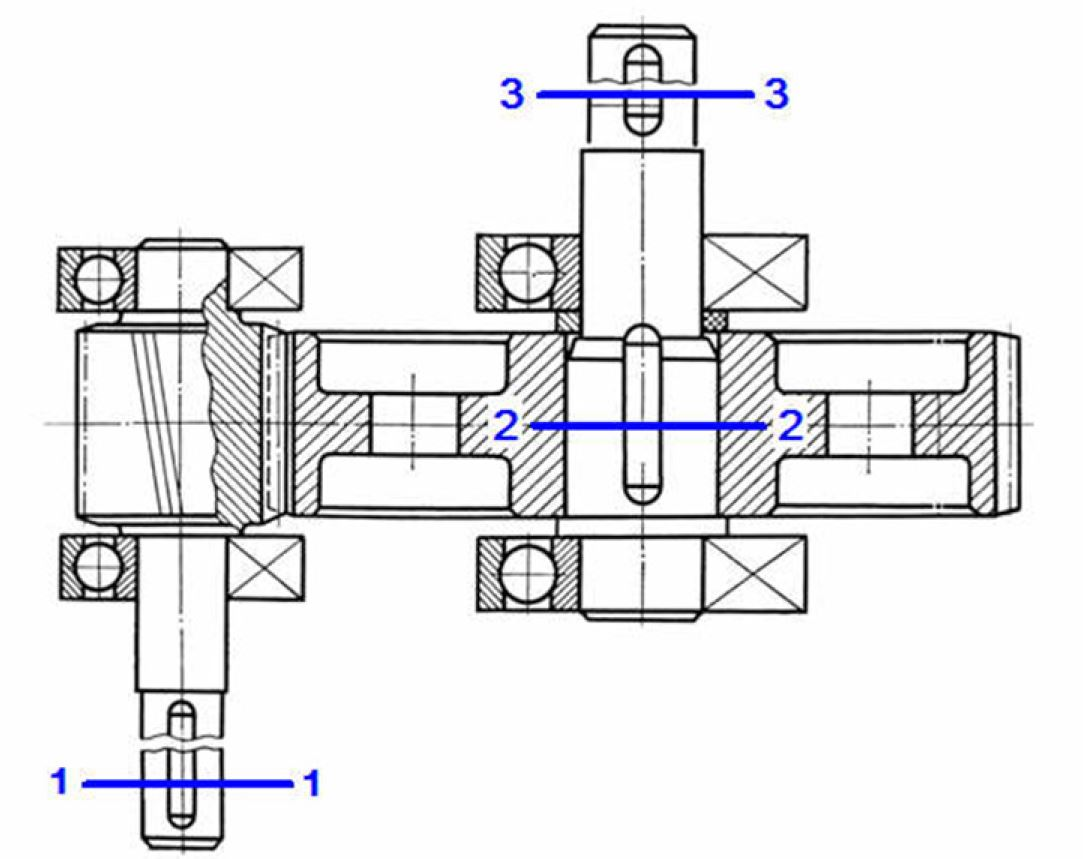
\includegraphics[width=1\textwidth]{KriticniPresjeci.jpg}
\caption{Kritični presjeci na vratilima reduktora}\label{fig:kriticniPresjeci}
\end{figure}

Na pogonskom vratilu provjera je izvšena u presjeku 1-1 (na spoju reduktora s pogonskim strojem) gdje je vratilo najtanje.
Na gonjenom vratilu reduktora provjera je izvršena na označenim presjecima 2-2 i 3-3.

Kontrolom na plastičnu deformaciju računa se koliko je puta granica tečenja $R_e$ ili $R_{p0,2}$ veća od najvećeg naprezanja.
Naprezanja se javljaju kao posljedica opterećenja $M_{s \, max}$, $F_{a \, max}$ i $T_{max}$.
Kao maksimana opterećenja uzeta su 3 puta veća on normalnih opterećenja koja se mogu javiti kod pokretanja ili zaustavljana stoja ili raznih udarnih opterećenja.
Faktor sigurnosti koji treba biti veći ili jedna 1.2 izračunat je pomoću sljedećeg izraza
\begin{equation}
S_p=\frac{1}{\sqrt{\left( \frac{\sigma_{s \, max}}{R_{es}}+\frac{\sigma_{v,tl \, max}}{R_e}\right)^2+ \left( \frac{\tau_{t \, max}}{R_{et}}\right)^2}}\geq 1,2 \label{equ_faktorSigurnostiPlasticeDeformacije}
\end{equation}
Stvarne granice tečenja su određene uzimajući u obzir tehnološki faktor $K_t$ zbog smanjenja granice tečenja s povećanjem promjera vratila zbog nehomogenosti materijala. Za korišteni materijal E360 (Č0745) korišten je izraz
\begin{equation}
K_t=1-0,26\cdot \log \left( \frac{D}{32} \right) \label{equ:faktorKt}
\end{equation}
Granice tečenja:
\begin{align}
R_e &= K_t \cdot R_{eN} \label{equ:Re} \\
R_{es} &= K_t \cdot R_{esN} \label{equ:Res} \\
R_{et} &= K_t \cdot R_{etN} \label{equ:Ret}
\end{align}
Pri čemu su $R_{eN}$, $R_{esN}$ i $R_{etN}$ su očitani iz tablice \cite{potrebniMaterijali}.

\subsubsection{presjek 1-1}
Uvrštavanjem podataka u \eqref{equ:faktorKt} dobiven je tehnološki faktor $K_t$
\begin{align*}
K_t&=1-0,26\cdot \log \left( \frac{D}{32} \right)\\
K_t&=1-0,26\cdot \log \left( \frac{105}{32} \right)\\
K_t&=\mathbf{0,8658}
\end{align*}
U presjeku 1-1 ne javljaju se vlačna niti tlačna opterećenja kao niti poterečenja koje uzrokuju savijenje ili su isti zanemarivo mali već postoji samo moment uvijanja koji uzrokuje torzijsko naprezanje.
Uvršavanjem poznatih podataka u \eqref{equ:Ret} dobivena je stvarna granica plastičnosti materijala pri torziji.
\begin{align*}
R_{et}&=0,8658 \cdot 250\\
R_{et}&=\mathbf{216 \dfrac{N}{mm^2}}
\end{align*}
Maksimalno torzijsko naprezanje koje se javlja u presjeku 1-1:
\begin{align*}
\tau_{t \, max}&=\frac{T_{max}}{W_p}=\frac{3 \cdot T_n \cdot 16}{(d-t_1)^3 \pi}\\
\tau_{t \, max}&=\frac{3 \cdot 121,5\cdot 10^3 \cdot 16}{(35)^3 \pi}\\
\tau_{t \, max}&=\mathbf{43,3 \dfrac{N}{mm^2}}
\end{align*}
Uvršavanjem poznatih podataka u \eqref{equ_faktorSigurnostiPlasticeDeformacije} dobiven je stvarni foktor sigurnosti
\begin{align*}
S_p&=\frac{1}{\sqrt{\left(\frac{43,3}{216}\right)^2}}\\
S_p&=\mathbf{4,99 > 1,2}
\end{align*}
Faktor sigurnosti u presjeku 1-1 zadovoljava postavljeni uvijet.

\subsubsection{presjek 2-2}
Uvrštavanjem podataka u \eqref{equ:faktorKt} dobiven je tehnološki faktor $K_t$
\begin{align*}
K_t&=1-0,26\cdot \log \left( \frac{D}{32} \right)\\
K_t&=1-0,26\cdot \log \left( \frac{80}{32} \right)\\
K_t&=\mathbf{0,8965}
\end{align*}
U presjeku 2-2 ne javljaju se vlačna niti tlačna opterećenja ili su isti zanemarivo mali već postoje samo moment uvijanja koji uzrokuje torzijsko naprezanje i sila na zupčanicima koja uzrokuje savijanje vratila izmeđe oslonaca (ležajeva).
Uvršavanjem poznatih podataka u \eqref{equ:Ret} dobivena je stvarna granica plastičnosti materijala pri torziji.
\begin{align*}
R_{et}&=0,8965 \cdot 250\\
R_{et}&=\mathbf{224 \dfrac{N}{mm^2}}
\end{align*}
Uvršavanjem poznatih podataka u \eqref{equ:Res} dobivena je stvarna granica plastičnosti materijala pri savijanju.
\begin{align*}
R_{es}&=0,8965 \cdot 430\\
R_{es}&=\mathbf{385,5 \dfrac{N}{mm^2}}
\end{align*}

Maksimalno torzijsko naprezanje koje se javlja u presjeku 2-2:
\begin{align*}
\tau_{t \, max}&=\frac{T_{max}}{W_p}=\frac{3 \cdot T_n \cdot 16}{(d-t_1)^3 \pi}\\
\tau_{t \, max}&=\frac{3 \cdot 462\cdot 10^3 \cdot 16}{(71)^3 \pi}\\
\tau_{t \, max}&=\mathbf{19,7 \dfrac{N}{mm^2}}
\end{align*}

Maksimalno naprezanje pri savijanju koje se javlja u presjeku 2-2:
\begin{align*}
\sigma_{s \, max}&=\frac{M_{s \, max}}{W}=\frac{3 \cdot M_s \cdot 32}{(d-t_1)^3 \pi}\\
\sigma_{s \, max}&=\frac{3 \cdot 74358,5  \cdot 16}{(71)^3 \pi}\\
\sigma_{s \, max}&=\mathbf{6,35 \dfrac{N}{mm^2}}
\end{align*}

Uvršavanjem poznatih podataka u \eqref{equ_faktorSigurnostiPlasticeDeformacije} dobiven je stvarni foktor sigurnosti
\begin{align*}
S_p&=\frac{1}{\sqrt{\left( \frac{6,35}{385,5}\right)^2+ \left(\frac{19,7}{224}\right)^2}}\\
S_p&=\mathbf{11,1 > 1,2}
\end{align*}
Faktor sigurnosti u presjeku 2-2 zadovoljava postavljeni uvijet.

\subsubsection{presjek 3-3}
Uvrštavanjem podataka u \eqref{equ:faktorKt} dobiven je tehnološki faktor $K_t$
\begin{align*}
K_t&=1-0,26\cdot \log \left( \frac{D}{32} \right)\\
K_t&=1-0,26\cdot \log \left( \frac{80}{32} \right)\\
K_t&=\mathbf{0,8965}
\end{align*}
U presjeku 3-3 ne javljaju se vlačna niti tlačna opterećenja kao niti poterečenja koje uzrokuju savijenje ili su isti zanemarivo mali već postoji samo moment uvijanja koji uzrokuje torzijsko naprezanje.
Uvršavanjem poznatih podataka u \eqref{equ:Ret} dobivena je stvarna granica plastičnosti materijala pri torziji.
\begin{align*}
R_{et}&=0,8965 \cdot 250\\
R_{et}&=\mathbf{224 \dfrac{N}{mm^2}}
\end{align*}
Maksimalno torzijsko naprezanje koje se javlja u presjeku 3-3:
\begin{align*}
\tau_{t \, max}&=\frac{T_{max}}{W_p}=\frac{3 \cdot T_n \cdot 16}{(d-t_1)^3 \pi}\\
\tau_{t \, max}&=\frac{3 \cdot 462\cdot 10^3 \cdot 16}{(53)^3 \pi}\\
\tau_{t \, max}&=\mathbf{47,4 \dfrac{N}{mm^2}}
\end{align*}
Uvršavanjem poznatih podataka u \eqref{equ_faktorSigurnostiPlasticeDeformacije} dobiven je stvarni foktor sigurnosti
\begin{align*}
S_p&=\frac{1}{\sqrt{\left(\frac{47,4}{224}\right)^2}}\\
S_p&=\mathbf{4,7 > 1,2}
\end{align*}
Faktor sigurnosti u presjeku 3-3 zadovoljava postavljeni uvijet.

\section{Proračun steznog spoja}
Dodirna površina između gonjenog vratila i zupčanika koji se navlači na njega je
\begin{align*}
A_F&=D_F \cdot l_F \cdot \pi \\
A_F&=84 \cdot 100 \cdot \pi \\
A_F&=\mathbf{26389,3 \, mm^2}
\end{align*}
Potrebna sila treba između zupčanika i vratila:
\begin{align*}
F_F&=\frac{2 \cdot T_2 \cdot \nu}{D_F}\\
F_F&=\frac{2 \cdot 462 \cdot 1,8}{84\cdot 10^{-3}}\\
F_F&=\mathbf{19800 \, N}
\end{align*}
Potrebna normalna sila usljed faktora trenja očitanog iz \cite{krivzan1998osnove}(tablica 9.11, str. 346.)
\begin{align*}
F_N&=\frac{F_F}{\mu}\\
F_N&=\frac{19800}{0,11}\\
F_N&=\mathbf{180000 \, N}
\end{align*}
Minimalni potrebni tlak steznog spoja:$$ p_{min}=\frac{F_N}{A_F} = \frac{180000}{26389,3}= \mathbf{6,82 \dfrac{N}{mm^2}}$$
Minimalni potrebni prijeklop je izračunat po izrazu
\begin{equation}
P_{st}=p \cdot D_F \cdot (K_V+K_U)\label{equ:Prijeklop}
\end{equation}
pri kojem su:
\begin{equation}
K_V=\frac{(m_V+1)+(m_V-1) \cdot Q_V^2}{m_V \cdot E_V \cdot (1-Q_V^2)}\label{equ:K_VFaktor}
\end{equation} i
\begin{equation}
K_U=\frac{m_U-1}{m_U \cdot E_U}\label{equ:K_UFaktor}
\end{equation}
gdje je $\nu=0,3$ - \textit{Poissonov} broj za čelik, $E=2,1 \cdot 10^5 \dfrac{N}{mm^2}$ - \textit{Youngov} modul elastičnosti za čelik, $m=\dfrac{1}{\nu}$, $Q_V=\dfrac{D_F}{D_V}$, $D_V\approx 2 \cdot D_F$.
Uvrštavanjem poznatih podataka u \eqref{equ:K_VFaktor} dobiven je faktor 
$$
K_V=\frac{(4,33)+(2,33) \cdot 0,5^2}{3,33 \cdot 2,1\cdot 10^5 \cdot (1-0,5^2)} \mathbf{= 9,36 \cdot 10^{-6} \, \dfrac{mm^2}{N}}
$$
Uvrštavanjem poznatih podataka u \eqref{equ:K_UFaktor} dobiven je faktor
$$
K_U=\frac{m_U-1}{m_U \cdot E_U}=\frac{2,33}{3,33 \cdot 2,1\cdot 10^5}\mathbf{= 3,33 \cdot 10^{-6} \, \dfrac{mm^2}{N}}
$$
Uvrštavanjem dobivenih faktora u \eqref{equ:Prijeklop} dobije se minimalni potrebni prijeklop
$$
P_{st}=6,82 \cdot 84 \cdot (9,36 \cdot 10^{-6} + 3,33 \cdot 10^{-6})= \mathbf{7,27 \, \mu m}
$$
Prilikom navlačenja zupčanika na vratilo pri čvrstom dosjedu dolazi do zaglađivanja hrapavosti površine. Zbog toga je potrebno povećati stvarni minimalni prijeklop po izrazu
\begin{equation}
P_{min}=P_{st}+3,2 \cdot (R_{a \, os}+R_{a \, gl})\label{equ:stvarniMinimalniPrijeklop}
\end{equation}
Pri čemu je $R_a$ - srednje aritmetičko odstupanje profila hrapavosti. Očitan iz \cite{krivzan1998osnove}(tablica 3.44, str 104) za kvalitetu obrade površine N7($R_{a(N7)}=1,6 \, \mu m$).
Uvrštavanjem dobivenih podataka u \eqref{equ:stvarniMinimalniPrijeklop} dobije se stvarni minimalni prijeklop
$$
P_{min}=\mathbf{17,51 \, \mu m}
$$
Maksimalni dopušteni tlak na steznoj površini je određen putem izraza
\begin{equation}
p_{max}\leq\frac{R_e \cdot (1-Q_V^2)}{1,2\cdot \sqrt{3+Q_V^4}}\label{equ:maxTlakSteznePovrsine}
\end{equation}
te uvrštavanjem poznatih podataka u izraz \eqref{equ:maxTlakSteznePovrsine} dobije se
$$
p_{max}\leq\frac{322 \cdot (1-0,5^2)}{1,2\cdot \sqrt{3+0,5^4}}=\mathbf{115 \, \dfrac{N}{mm^2}}
$$
Stvarni dopušteni maksimalni prijeklop po izrazu \eqref{equ:Prijeklop} iznosi
$$
P_{max}=115 \cdot 84 \cdot (9,36 \cdot 10^{-6} + 3,33 \cdot 10^{-6})= \mathbf{122,58 \, \mu m}
$$
\textbf{TREBA ODABRATI TOLERANCIJSKA POLJA ZA ČVRSTI DOSJED PREMA DOBIVENIM PODACIMA}

\section{Proračun valjnih ležajeva}
Trajnost ležajeva se može proračunati po izrazu
\begin{equation}
L_{10h}=\left(\frac{C}{F} \cdot f_t \right)^p \cdot \frac{10^6}{60 \cdot n}
\label{equ:trajnostLezaja}
\end{equation}
pri čemu je $C$ - dinamička nosivost ležaja, $p$ - eksponent vijeka trajanja. Za kuglične ležajeve $p=3$, za ostale $p=\dfrac{10}{3}$ i $f_t$ - temperaturni faktor. Za $\vartheta < 150^\circ C \Rightarrow f_t=1$.

Odabrani ležajevi za pogonsko vratilo imaju dinamičku nosivost $C=17,8 \,kN$.
Uvršavanje poznatih podataka u \eqref{equ:trajnostLezaja} dobije se minimalna trajnost ležaja
\begin{align*}
L_{10h1}&=\left(\frac{17800}{1231} \cdot 1 \right)^3 \cdot \frac{10^6}{60 \cdot 1100}\\
L_{10h1}&=\mathbf{45808\, h}
\end{align*}
Odabrani ležaj zadovoljava potrebnu minimalnu trajnost iz zahtjeva.

Odabrani ležajevi za gonjeno vratilo imaju dinamičku nosivost $C=54,7 \,kN$.
Uvršavanje poznatih podataka u \eqref{equ:trajnostLezaja} dobije se minimalna trajnost ležaja
\begin{align*}
L_{10h2}&=\left(\frac{54700}{1171} \cdot 1 \right)^{\dfrac{10}{3}} \cdot \frac{10^6}{60 \cdot 275}\\
L_{10h2}&=\mathbf{22247650\, h}
\end{align*}
Odabrani ležaj zadovoljava potrebnu minimalnu trajnost iz zahtjeva.

Tehnički podaci odabranog ležaja za pogonsko vratilo se nalazi na slici \ref{fig:lezajPogonskogVratila}.
\begin{figure}
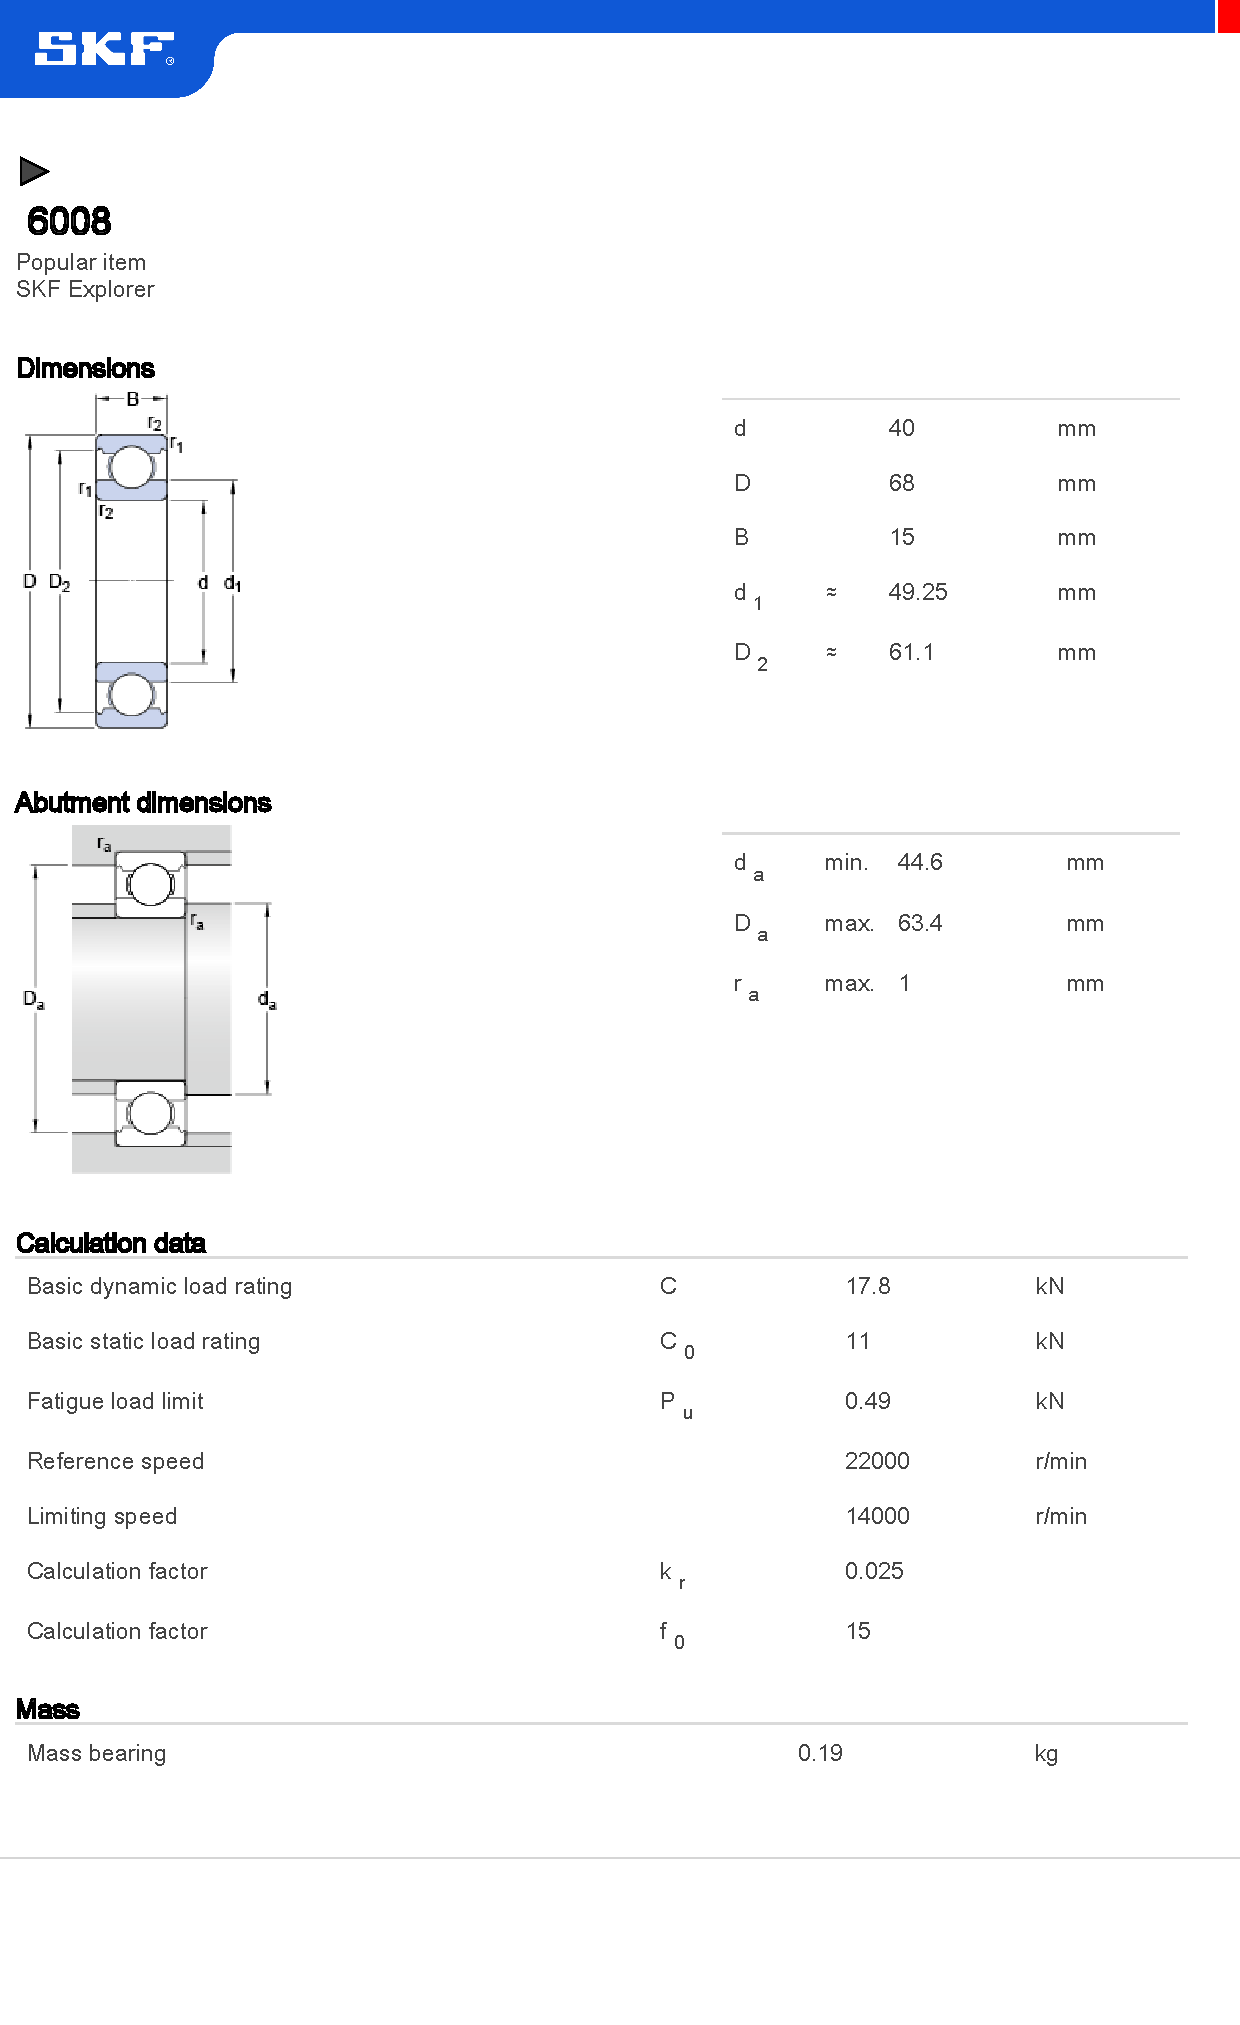
\includegraphics[width=1\textwidth]{datasheetsModels/Deep_groove_ball_bearings-6008.pdf}
\caption{Tehnički podaci ležaja pogonskog vratila SKF 6008}\label{fig:lezajPogonskogVratila}
\end{figure} 
Tehnički podaci odabranog ležaja za gonjeno vratilo se nalazi na slici \ref{fig:lezajGonjenogVratila}
\begin{figure}[h]
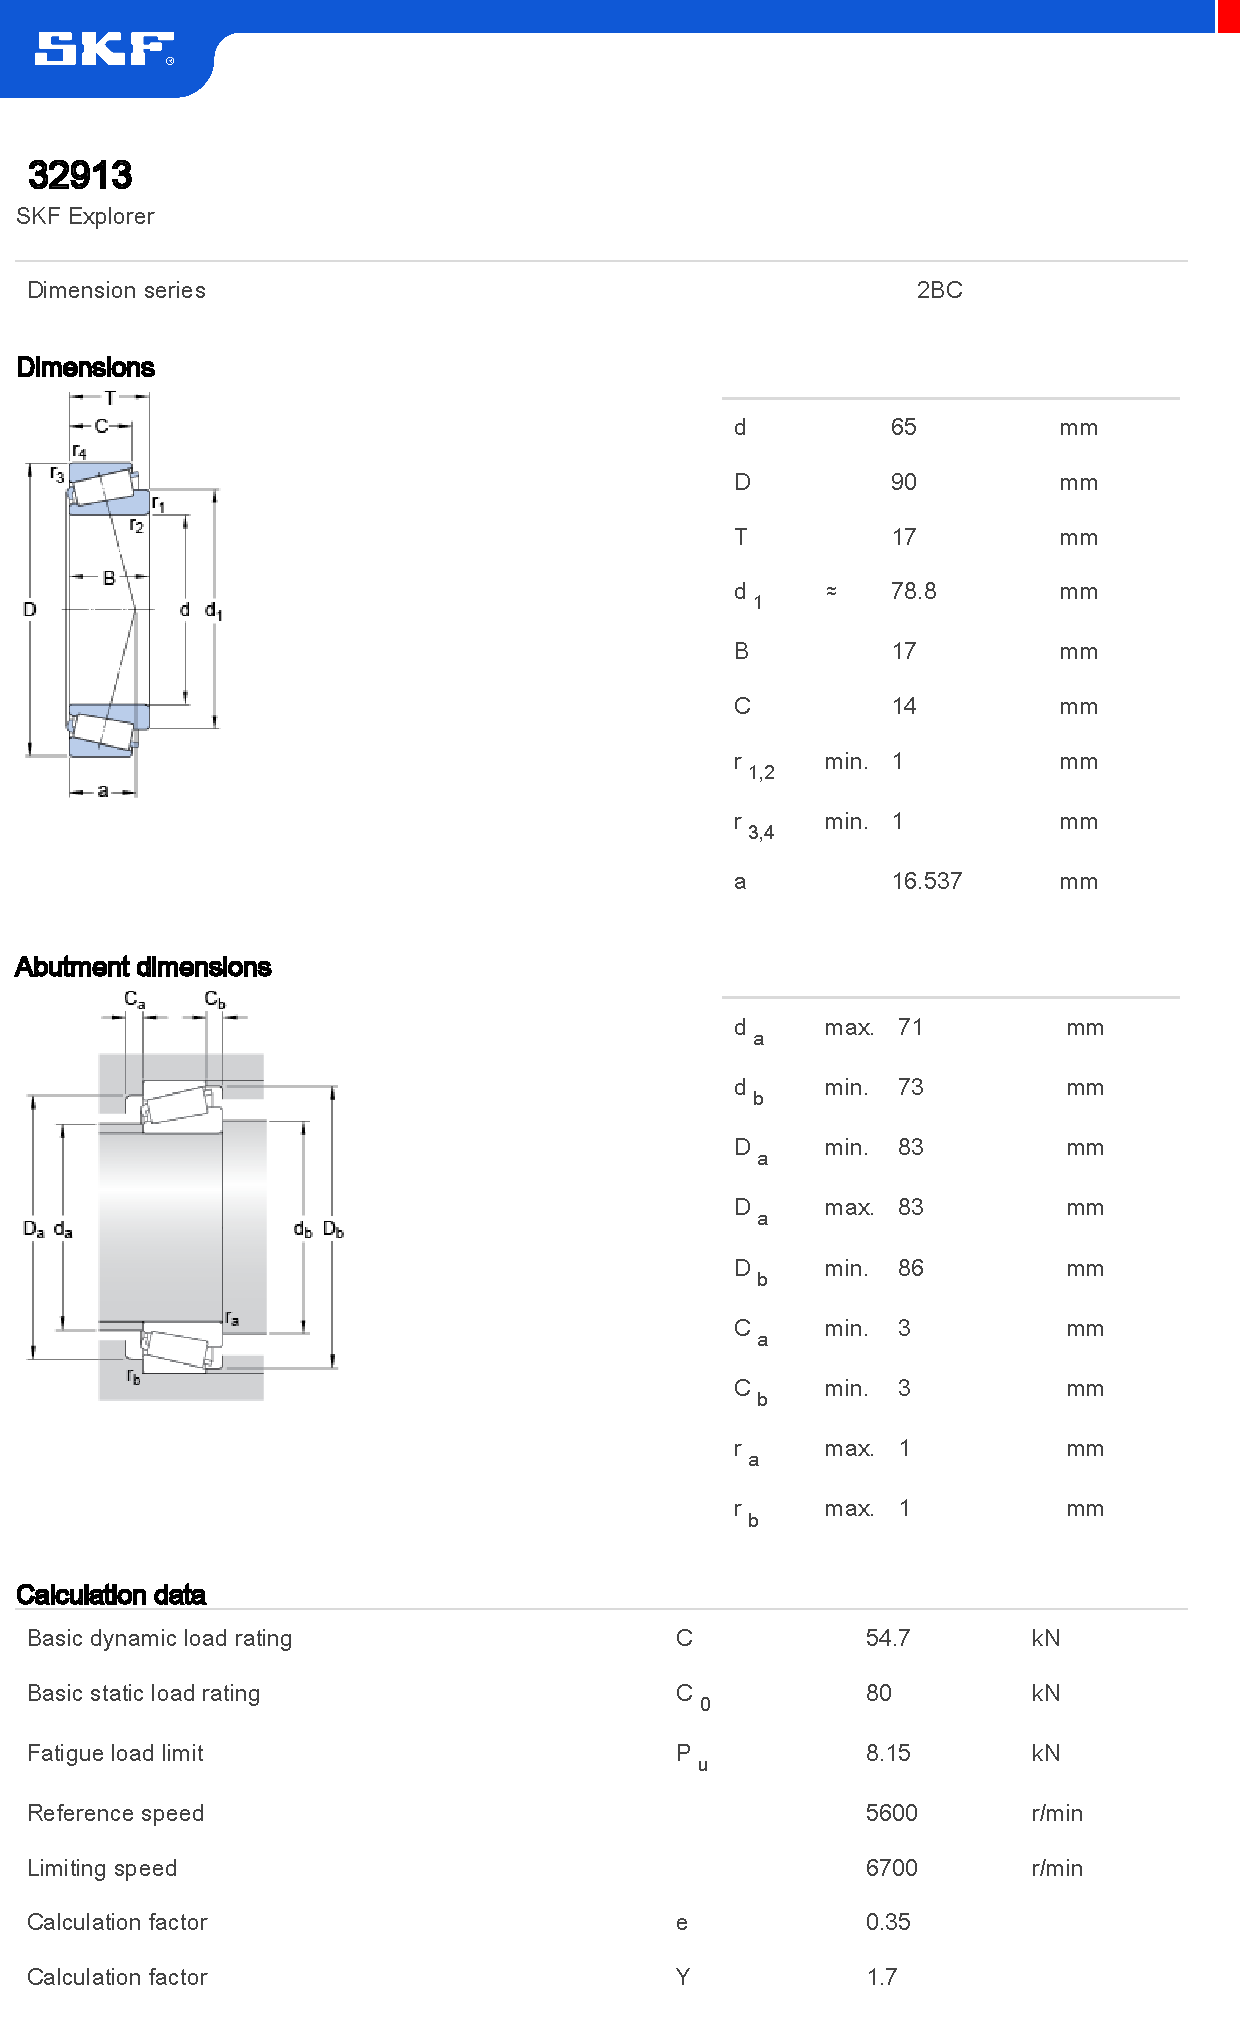
\includegraphics[width=1\textwidth]{datasheetsModels/Tapered_roller_bearings_single_row-32913.pdf}
\caption{Tehnički podaci ležaja pogonskog vratila SKF 32913}\label{fig:lezajGonjenogVratila}
\end{figure}


\newpage
\nocite{*}
\addcontentsline{toc}{chapter}{Literatura}
\bibliography{literatura}

\newpage
\appendix
\addcontentsline{toc}{chapter}{Dodatak A: Radionički nacrt pogonskog vratila}
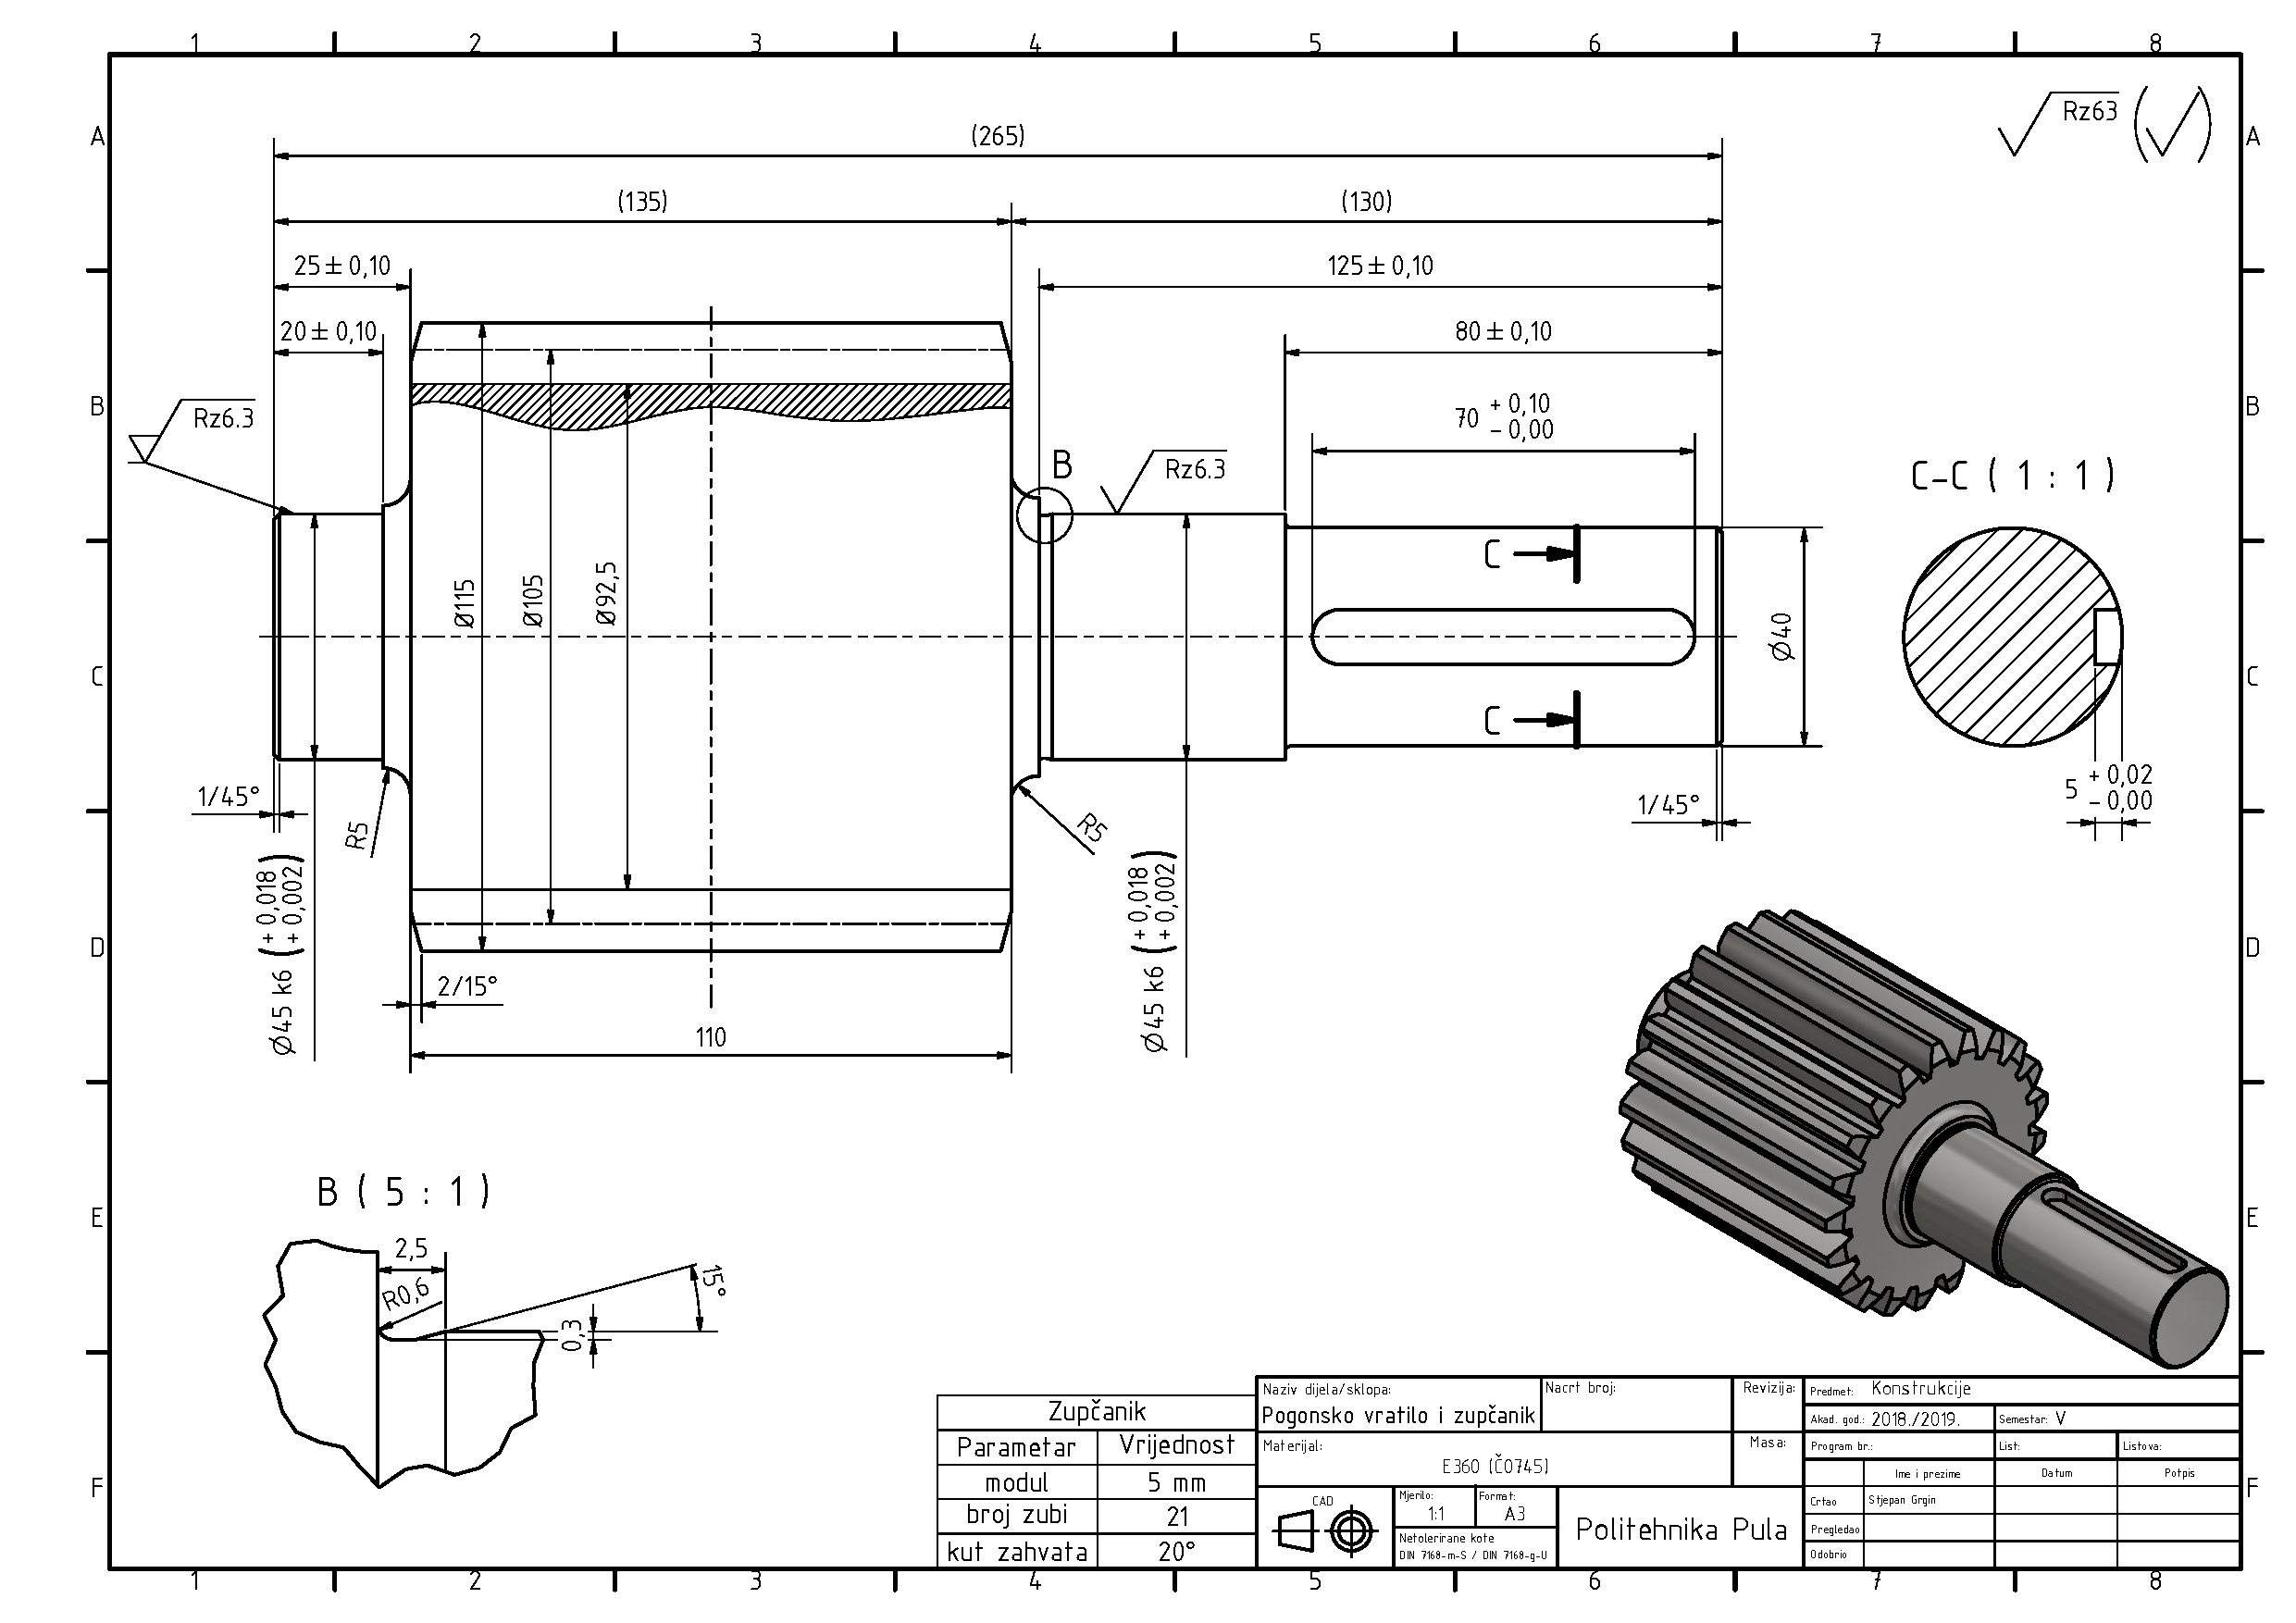
\includepdf[fitpaper]{OutputDrawings/PogonskoVratilo.pdf}
\addcontentsline{toc}{chapter}{Dodatak B: Radionički nacrt gonjenog vratila}
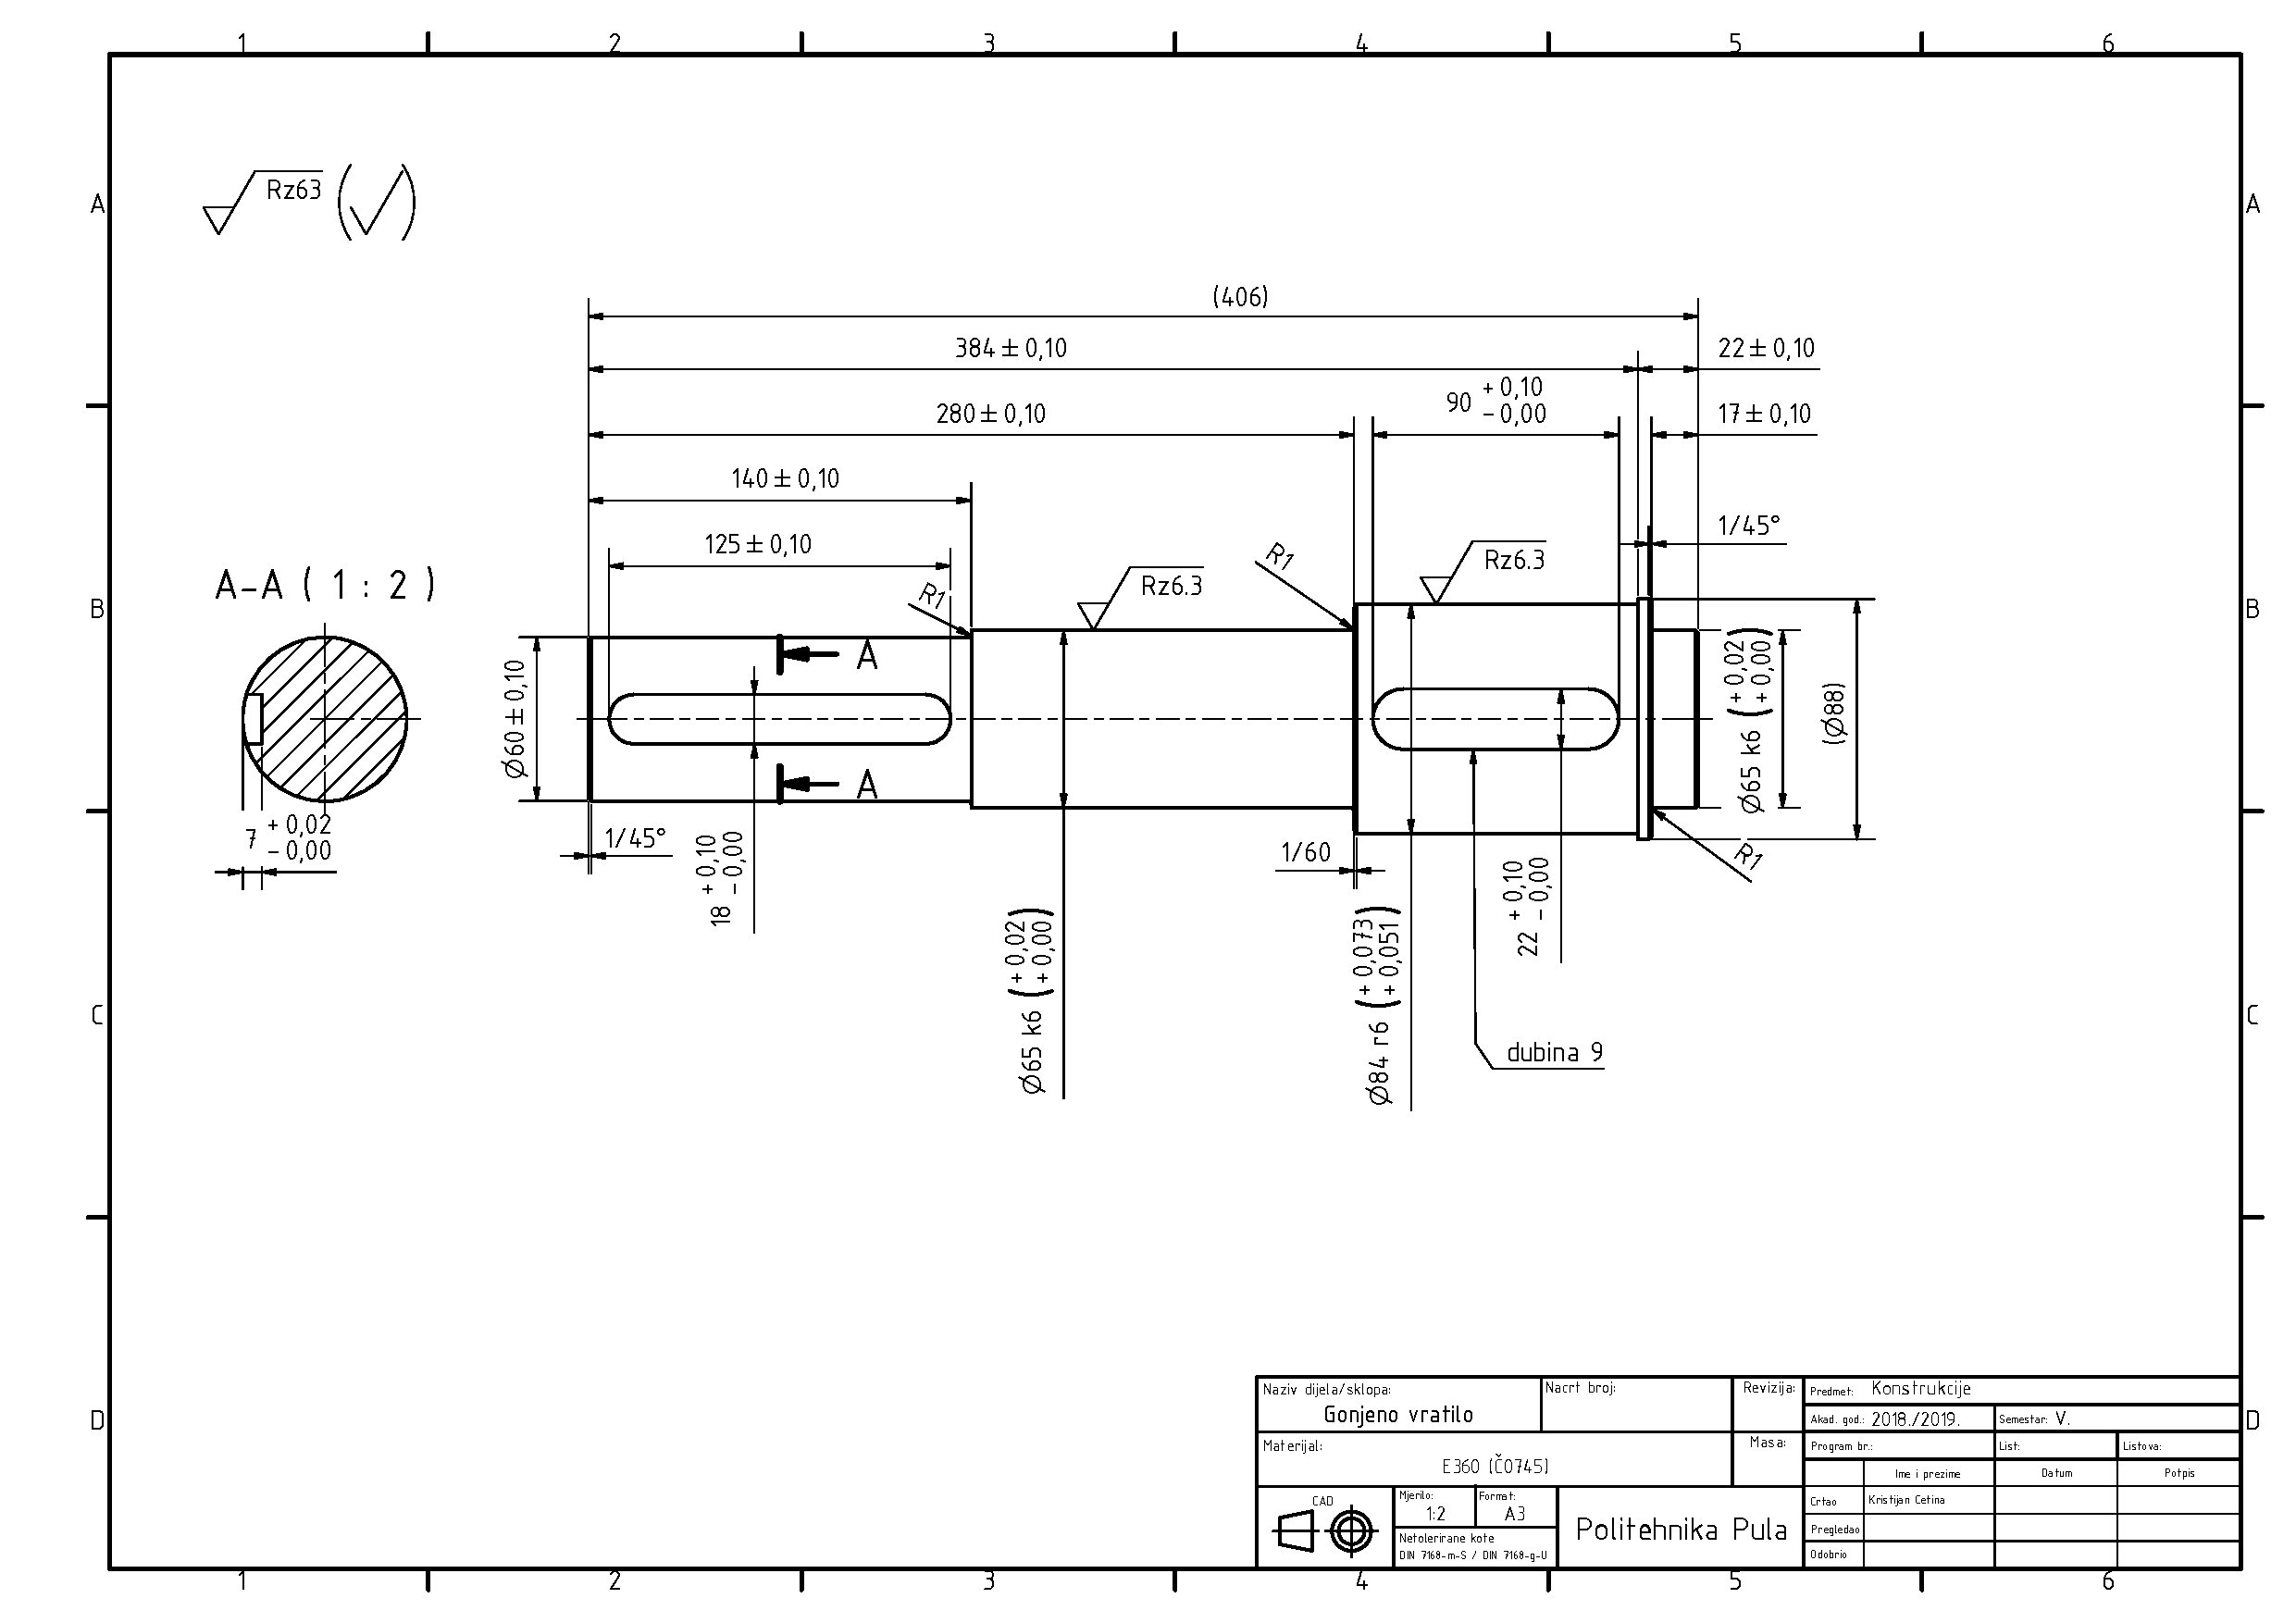
\includepdf[fitpaper]{OutputDrawings/GonjenoVratilo.pdf}
\end{document}